% SC4023 --- Chapter 4: Automated Program Repair (0->100 ground-up)
\chapter{Automated Program Repair}
\label{ch:repair}
\sloppy

\begin{quote}
\emph{``Fixing a bug is not just changing a line; it is arguing that the new line is more correct than the old one.''} --- Automated repair makes that argument executable: generate a candidate, show that it passes the tests, and invite human judgement on whether the argument holds.
\end{quote}

\noindent\fbox{\parbox{\dimexpr\linewidth-2\fboxsep-2\fboxrule}{%
\textbf{From zero: no repair background assumed.} We start from a failing test and the question ``what would make it pass?''---how to find where the bug lives, how to propose a change, and how to check the change does not break something else. Every technique is shown as picture, then rule, then example.}}
\vspace{0.4em}

\section*{Learning Outcomes}
After this chapter you will be able to:
\begin{enumerate}[label=(L\arabic*)]
    \item define fault localisation, patch generation, and validation;
    \item trace the GenProg loop (evolutionary search over patches);
    \item explain template-based and learning-based repair (TBar, SequenceR);
    \item distinguish plausible from correct patches and overfitting;
    \item evaluate a repair tool with standard metrics and benchmarks.
\end{enumerate}

% ============================================================
\section{What Is Automated Program Repair?}
\label{sec:what-is-apr}
\paragraph{Intuition.} You have a program $P$, a test suite $T$ where at least one test fails, and you want a program $P'$ that passes all of $T$ and does not introduce new failures. The search space is enormous---every possible edit to $P$---so repair techniques differ in how they narrow it: heuristic search, fixed templates, or learned patterns from past fixes.

The standard pipeline has three stages. \emph{Fault localisation} ranks suspicious lines (often with spectrum-based scoring: lines executed mostly by failing tests rank high). \emph{Patch generation} proposes edits at those lines. \emph{Validation} runs $T$ (and sometimes extra generated tests) to keep only \emph{plausible} patches---those passing $T$. A plausible patch is not necessarily \emph{correct}; it may overfit to the tests.

\begin{figure}[h]\centering
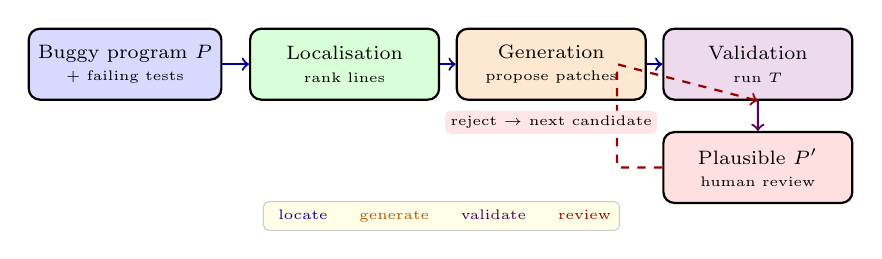
\begin{tikzpicture}[scale=0.82,every node/.style={font=\scriptsize},
  box/.style={draw,thick,rounded corners=4pt,minimum width=2.4cm,minimum height=0.9cm,align=center}]
  \node[box,fill=blue!15] (bug) at (0,0) {Buggy program $P$\\\tiny + failing tests};
  \node[box,fill=green!15] (loc) at (3.4,0) {Localisation\\\tiny rank lines};
  \node[box,fill=orange!18] (gen) at (6.6,0) {Generation\\\tiny propose patches};
  \node[box,fill=violet!14] (val) at (9.8,0) {Validation\\\tiny run $T$};
  \node[box,fill=red!12] (patch) at (9.8,-1.6) {Plausible $P'$\\\tiny human review};
  \foreach \a/\b in {bug/loc,loc/gen,gen/val}
    \draw[->,thick,blue!60!black] (\a) -- (\b);
  \draw[->,thick,violet!70!black] (val) -- (patch);
  \draw[->,thick,red!60!black,dashed] (patch.west) -- ++(-0.7,0) -- ++(0,1.6) -- (val.south);
  \node[font=\tiny,fill=red!10,rounded corners=2pt,inner sep=2pt] at (6.6,-0.9) {reject $\to$ next candidate};
  \node[font=\tiny,align=left,fill=yellow!10,draw=gray!40,rounded corners=2pt,inner sep=3pt] at (4.9,-2.35) {\textcolor{blue!60!black}{$\blacksquare$ locate} \quad \textcolor{orange!70!black}{$\blacksquare$ generate} \quad \textcolor{violet!60!black}{$\blacksquare$ validate} \quad \textcolor{red!60!black}{$\blacksquare$ review}};
\end{tikzpicture}
\caption{The APR pipeline. Localisation narrows \emph{where}; generation proposes \emph{what}; validation checks against $T$. Only plausible patches reach human review, and review decides correctness.}
\label{fig:apr-pipeline}
\end{figure}

\begin{definition}[Plausible vs.\ correct]
A \emph{plausible} patch passes all tests in $T$. A \emph{correct} patch is plausible and also satisfies the intended specification (what the developer meant). Overfitting---passing $T$ while violating the spec---is the central failure mode of APR.
\end{definition}

Small example: \texttt{if (x > 0) y=1/x;} with test \texttt{x=0 should not crash}. The empty fix \texttt{if (true) y=0;} passes the test but is not correct; a correct fix guards the division.

\begin{example}[Spectrum-based localisation]
Suppose line $L_1$ is executed by 3 failing and 1 passing test, $L_2$ by 0 failing and 4 passing. Ochiai score $s(L)=\frac{\text{failed}(L)}{\sqrt{(\text{failed}(L)+\text{passed}(L))\cdot \text{totalFailed}}}$ ranks $L_1$ much higher. The intuition is simple: suspiciousness grows with failing coverage and shrinks with passing coverage.
\end{example}

% ============================================================
\section{GenProg and Search-Based Repair}
\label{sec:genprog}
\paragraph{Intuition.} If you do not know the right fix, try many small edits and keep those that get closer to passing. GenProg treats a program as a genome: \emph{mutation} changes a line, \emph{crossover} swaps edits between candidates, and \emph{fitness} is the number of tests passed.

Concretely, GenProg starts from $P$, localises suspicious statements, and creates a population of variants by copying, deleting, or swapping statements drawn from elsewhere in the program (the \emph{plastic surgery hypothesis}: the fix ingredient often exists nearby). Each variant is executed on $T$; fitter variants breed the next generation. When a plausible patch appears, the search stops and the patch is minimised (redundant edits removed).

\begin{figure}[h]\centering
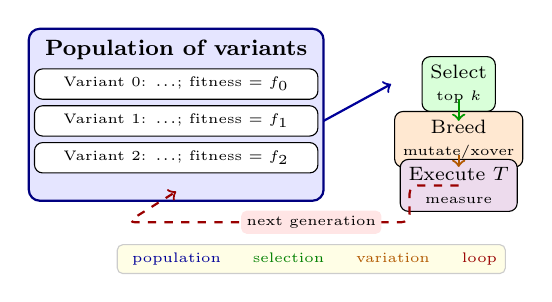
\begin{tikzpicture}[scale=0.78,every node/.style={font=\scriptsize}]
  \draw[fill=blue!10,draw=blue!50!black,thick,rounded corners=4pt] (0,0) rectangle (4.8,2.8);
  \node[font=\footnotesize\bfseries] at (2.4,2.45) {Population of variants};
  \foreach \i/\y in {0/1.9,1/1.3,2/0.7} {
    \node[draw,fill=white,rounded corners=3pt,minimum width=3.6cm,align=left,inner sep=3pt] at (2.4,\y) {\tiny Variant \i: \texttt{...}; fitness $=f_\i$};
  }
  \node[draw,fill=green!15,rounded corners=3pt,inner sep=3pt,align=center] at (7.0,1.9) {Select\\\tiny top $k$};
  \node[draw,fill=orange!18,rounded corners=3pt,inner sep=3pt,align=center] at (7.0,1.0) {Breed\\\tiny mutate/xover};
  \node[draw,fill=violet!14,rounded corners=3pt,inner sep=3pt,align=center] at (7.0,0.25) {Execute $T$\\\tiny measure};
  \draw[->,thick,blue!60!black] (4.8,1.3) -- (5.9,1.9);
  \draw[->,thick,green!60!black] (7.0,1.65) -- (7.0,1.30);
  \draw[->,thick,orange!70!black] (7.0,0.75) -- (7.0,0.55);
  \draw[->,thick,red!60!black,dashed,rounded corners=3pt] (7.0,0.25) -- ++(-0.8,0) -- ++(0,-0.6) -- ++(-4.6,0) -- (2.4,0.15);
  \node[font=\tiny,fill=red!10,rounded corners=2pt,inner sep=2pt] at (4.6,-0.35) {next generation};
  \node[font=\tiny,align=left,fill=yellow!10,draw=gray!40,rounded corners=2pt,inner sep=3pt] at (4.6,-0.95) {\textcolor{blue!60!black}{$\blacksquare$ population} \quad \textcolor{green!50!black}{$\blacksquare$ selection} \quad \textcolor{orange!70!black}{$\blacksquare$ variation} \quad \textcolor{red!60!black}{$\blacksquare$ loop}};
\end{tikzpicture}
\caption{GenProg as evolutionary search. Fitness is tests passed; mutation and crossover propose nearby programs; selection keeps the fittest. The loop is a direct analogue of generate--execute--filter from testing.}
\label{fig:genprog}
\end{figure}

GenProg was the first to fix real C bugs automatically (e.g., in \texttt{libtiff}, \texttt{php}) with no hand-written templates. Its strength is generality; its weakness is that random edits rarely produce a correct multi-line fix and the search is expensive.

\paragraph{Why plastic surgery works (and when it does not).} Large codebases are repetitive: error handling, null checks, and boundary conditions appear many times in slightly different forms. Copying a nearby correct snippet is often enough for small bugs. It fails when the needed code does not already exist in the project (novel logic) or when the fix requires coordinated changes across files, which single-statement edits cannot express.

\begin{example}[A GenProg-style fix]
Buggy: \texttt{if (x != 0) y = 1/x; else y = 0;} with test \texttt{x=0 => y=0} passes but \texttt{x=0.0} still divides by zero due to typed comparison. A variant that copies a null-guard from nearby---\texttt{if (x==0) y=0; else y=1/x;}---is found by mutation and scores higher.
\end{example}

% ============================================================
\section{Learning Fix Patterns: From TBar to SequenceR}
\label{sec:learned-repair}
Search is general but blind; learning makes it sighted. \emph{Template-based} repair (e.g., TBar) mines common fix templates from human patches---null-check insertion, bound adjustment, operator swap---and tries those first at suspicious locations. \emph{Neural} repair (e.g., SequenceR, Recoder, AlphaRepair) trains a seq2seq or LLM to translate buggy code into fixed code, learning from millions of before--after pairs.

\begin{lstlisting}[language=Java, caption={Template vs.\ learned fix: the same null dereference repaired two ways.}, label={lst:template-fix}]
// Buggy Java: null dereference on line 3
String greet(String name) {
    int len = name.length(); // NPE if name == null
    return "Hello " + name;
}
// Template fix (TBar: Insert null check)
String greet(String name) {
    if (name == null) return "Hello guest";
    int len = name.length();
    return "Hello " + name;
}
// Neural fix might instead produce:
// if (name == null) name = "guest";  // learned variant
\end{lstlisting}

The workflow for neural repair: input is the buggy snippet plus surrounding context and an error message; the model outputs a patch (often as a diff). Decoding is done with beam search; top-$k$ patches are validated against $T$. Training data is mined from GitHub commits whose messages contain ``fix'' and whose diff is small. A crucial detail is \emph{context}: the same buggy line may need different fixes depending on imports, types, and nearby methods, so modern models include a window of surrounding code, not just the single line.

\paragraph{Bias in learned fixes.} Models reproduce what they have seen most: if training data contains many null-check insertions, the model will propose null checks even when a bound check is correct. Diversity in training fixes and explicit ranking by test outcome (not just likelihood) help, but the bias remains. This is why hybrid systems that try templates first and fall back to neural sampling often outperform pure neural approaches.

\begin{lstlisting}[language=Python, caption={Python: off-by-one fix as a one-token change. A model that has seen many such pairs learns the pattern.}, label={lst:off-by-one}]
# Buggy
def sum_range(arr, lo, hi):
    s = 0
    for i in range(lo, hi):  # bug: should be hi+1 if inclusive
        s += arr[i]
    return s

# Fixed (inclusive upper bound)
def sum_range(arr, lo, hi):
    s = 0
    for i in range(lo, hi+1):
        s += arr[i]
    return s
# Test that distinguishes: sum_range([1,2,3],0,2) should be 6
\end{lstlisting}

\begin{figure}[h]\centering
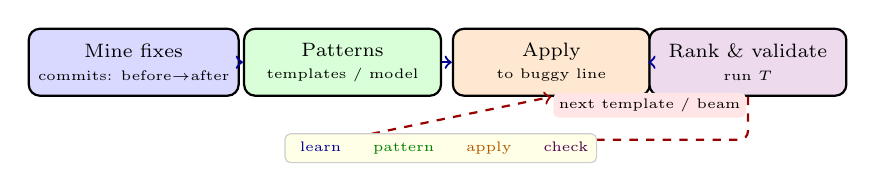
\begin{tikzpicture}[scale=0.78,every node/.style={font=\scriptsize},
  box/.style={draw,thick,rounded corners=4pt,minimum width=2.5cm,minimum height=0.85cm,align=center}]
  \node[box,fill=blue!15] (mine) at (0,0) {Mine fixes\\\tiny commits: before$\to$after};
  \node[box,fill=green!15] (pat) at (3.4,0) {Patterns\\\tiny templates / model};
  \node[box,fill=orange!18] (apply) at (6.8,0) {Apply\\\tiny to buggy line};
  \node[box,fill=violet!14] (rank) at (10.0,0) {Rank \& validate\\\tiny run $T$};
  \foreach \a/\b in {mine/pat,pat/apply,apply/rank}
    \draw[->,thick,blue!60!black] (\a) -- (\b);
  \draw[->,thick,red!60!black,dashed,rounded corners=3pt] (rank.south) -- ++(0,-0.7) -- ++(-6.6,0) -- (apply.south);
  \node[font=\tiny,fill=red!10,rounded corners=2pt,inner sep=2pt] at (8.4,-0.7) {next template / beam};
  \node[font=\tiny,align=left,fill=yellow!10,draw=gray!40,rounded corners=2pt,inner sep=3pt] at (5.0,-1.4) {\textcolor{blue!60!black}{$\blacksquare$ learn} \quad \textcolor{green!50!black}{$\blacksquare$ pattern} \quad \textcolor{orange!70!black}{$\blacksquare$ apply} \quad \textcolor{violet!60!black}{$\blacksquare$ check}};
\end{tikzpicture}
\caption{Learning fix patterns. Past fixes are mined into templates or a neural model; at repair time the model proposes patches at localised lines and they are ranked by validation on $T$.}
\label{fig:learned-repair}
\end{figure}

Learning helps with common, local fixes (one--two lines, familiar APIs) and struggles with novel, multi-file, or specification-heavy bugs. The best recent systems hybridise: templates handle known patterns quickly, neural models handle the long tail, and search fills gaps when both miss.

\paragraph{Context is critical.} The same buggy line \texttt{name.length()} needs different fixes depending on whether \texttt{name} is allowed to be null (add guard) or should never be null (fix the caller). Modern neural repair models therefore feed the model not just the buggy line but a window of surrounding method, the failing test message, and sometimes the stack trace. Without that context, even a perfect learner guesses.

\begin{example}[How much context matters]
With only the line \texttt{int len = name.length();}, a model cannot know whether the intended fix is \texttt{if (name==null) return 0;} or \texttt{if (name==null) name="";}. With the caller \texttt{greet(null)} and test \texttt{assertEquals("Hello guest", greet(null))} in context, the second is clearly preferred. This is why APR is increasingly framed as \emph{retrieval-augmented generation}: fetch relevant tests and docs, then generate.
\end{example}

A useful analogy: template repair is a phrasebook (fast for known phrases), neural repair is a fluent speaker (general but occasionally wrong), and search is trial-and-error (slow but needs no prior knowledge). Good pipelines try them in that order.

In practice, teams combine all three: mine templates from the project's own history, fine-tune a neural model on that history, and fall back to search when both fail. The shared bottleneck remains validation---without strong tests, every approach overfits.

% ============================================================
\section{Evaluation, Overfitting, and Limits}
\label{sec:eval-repair}
A repair tool is judged by \emph{plausible rate}, \emph{correct rate} (human-judged), and \emph{precision} (correct/plausible). Benchmarks like \emph{Defects4J} (Java, 800+ real bugs), \emph{ManyBugs} (C), and \emph{QuixBugs} provide $P$ and $T$; leakage and weak $T$ are constant threats. Tools often report ``$X$ bugs fixed'' without distinguishing plausible from correct---always check which number is quoted.

The central pitfall is \emph{test overfitting}: a patch that deletes functionality can pass a weak suite (e.g., removing the feature that has the bug). Mitigations include augmenting $T$ with generated tests (as in Ch.~3), checking against a held-out oracle when available, and requiring minimal edits. In practice, combining a weak APR patch with one human-written regression test often turns a plausible patch into a correct one.

\begin{definition}[Overfitting in repair]
A patch \emph{overfits} $T$ if it passes $T$ but fails outside it---it fits the tests, not the spec. Stronger validation (more tests, not more search) is the primary defence. Two common overfit patterns are \emph{test-suite overfitting} (the patch hard-codes the expected output for a specific test input) and \emph{incomplete fixing} (it repairs one failing test while breaking an untested behaviour).
\end{definition}

\begin{remark}[What repair cannot do]
APR is best at small, local, pattern-following fixes where tests are strong---typically one to three lines in a single method. It is not a substitute for understanding the specification. For a novel feature or a design flaw, the correct action is to clarify the spec and write the code deliberately---the assistant proposes, the engineer decides, as in every chapter.
\end{remark}

% ============================================================
\section{Chapter Notes}
GenProg (Le Goues et~al., 2012) founded search-based repair; Defects4J (Just et~al., 2014) standardised evaluation. TBar (Liu et~al., 2019) systematised template mining; SequenceR (Chen et~al., 2019), Recoder, and AlphaRepair represent the neural line. The overfitting analysis of Qi et~al.\ and Smith et~al.\ is essential reading on why plausible $\neq$ correct and how augmented testing helps. Recent surveys (Goues et~al., 2022; Zhang et~al., 2023) map the full design space of localisation, generation, and validation choices.

\begin{remark}[Practical tip]
When triaging a tool's patch, ask: does it generalise beyond the failing test? A quick check is to write one more test that the fix should satisfy but the buggy code did not (e.g., \texttt{greet("")} or \texttt{greet("A very long name")} ). If the patch fails that new test, it likely overfits.
\end{remark}

% ============================================================
\section{Exercises}
\label{sec:ch04-exercises}
\begin{enumerate}[label=E4.\arabic*, leftmargin=*, itemsep=0.7em]
    \item \textbf{Pipeline.} For a buggy \texttt{median} that returns wrong output on even-length lists, walk through Fig.~\ref{fig:apr-pipeline}: which lines would spectrum-based localisation rank highest? What templates would TBar try first? How would validation decide?
    \item \textbf{GenProg fitness.} A suite has 10 tests, 3 failing on $P$. Variant $A$ passes 8 tests, variant $B$ passes 7 but fixes one previously failing test while breaking a previously passing one. Which has higher fitness? Which would you prefer to breed from? Propose a fitness that rewards fixing failing tests more than preserving passing ones.
    \item \textbf{Template vs.\ neural.} Give a bug where a template is likely to succeed and one where a neural model might succeed while templates fail. Justify each in one sentence by referring to fix locality and pattern frequency.
    \item \textbf{Overfitting.} A repair deletes the buggy method body and returns a constant that happens to pass all existing tests. Explain why this is plausible but not correct. Propose two concrete additions to $T$ that would reject it: one coverage-guided test and one metamorphic test.
    \item \textbf{Hands-on.} Take the Java \texttt{greet} bug in Listing~\ref{lst:template-fix}. Prompt any LLM with the buggy method plus the failing test \texttt{assertEquals("Hello guest", greet(null))} and ask for a minimal fix. Validate the patch by running the test. Is the patch plausible? Is it correct for all callers? Argue in two sentences.
\end{enumerate}
% End of Chapter 4
